\subsection{BPMS: Camunda}
Il meccanismo di interazione tra il sistema (in altre parole, l'azienda
ACME) e l'utente \`e stata gestita tramite la piattaforma Camunda.
Si sono creati due progetti:
\begin{enumerate}
  \item {\tt CamundaProject};
  \item {\tt UserWebEndPoint}.
\end{enumerate}
{\tt CamundaProject} contiene il diagramma BPMN, creato grazie al
software {\it Camunda Modeler}, l'implementazione Java delle azioni
descritte nel diagramma stesso  e i form che permettono di dare un
formato regolare alle richieste degli utenti. In altre parole,
implementa la logica del server.
{\tt UserWebEndpoint} contiene invece una {\it servlet} che permette di
lanciare i processi (cio\`e, in questo caso, gli ordini).

La servlet implementata \`e la {\tt SendOrderRequest}, che simula
l'invio di un ordine da parte di un utente al sistema. Esistono tre
tipologie di ordini possibili, mappate attraverso il parametro
{\tt value}:
\begin{enumerate}
  \item ordine contenente {\it n} cicli, con $n > 0$;
  \item ordine contenente {\it n} componenti, con $n > 0$;
  \item ordine contenente {\it n} cicli e $m$ componenti, con
  $n > 0 \land m > 0$.
\end{enumerate}
L'ordine viene implementato attraverso un messaggio.
Le prime due tipologie di ordine contengono una lista di
customizzazioni: per esempio la customizzazione di un componente
potrebbe essere il colore del componente stesso.

L'invio del messaggio di avvio a Camunda \`e possibile perch\'e siamo
sullo stesso server: si applica infatti la tecnica {\it injection}, che
permette di prendere una risorsa interna al server ed ``iniettarla''
all'interno del processo.
In questo caso viene iniettata una variabile di tipo
{\tt ProcessEngine}, che \`e una risorsa di Camunda: tale variabile
viene utilizzata per inviare il messaggio a tutti i servizi in attesa:
se esso contiene l'id {\tt start}, il servizio che lo riceve istanzia un
processo.

Si esaminano ora i vari passaggi effettuati dal processo, dalla
ricezione \linebreak dell'ordine fino alla sua conclusione.

Per prima cosa viene analizzata la tipologia di ordine: se \`e della
terza tipologia indicata in precedenza, genera tanti messaggi quanti
sono gli ordini presenti e lancia un ugual numero di processi. Fatto
ci\`o termina. Se invece si ha a che fare con un ordine singolo, si
procede.

Si controlla la presenza di customizzazioni, seguendo i passaggi
indicati nel diagramma BPMN. \`E importante notare che il processo
memorizza le informazioni legate all'ordine all'interno di variabili
d'ambiente. Il controllo sulla compatibilit\`a delle customizzazioni
viene effettuata tramite una decisione pseudo-randomica (con una
probabilit\`a di successo del 90\%), presa su tutto l'insieme delle
customizzazioni.

Dopo aver controllato la tipologia di ordine, il sistema si comporta
come descritto nel diagramma BPMN; successivamente viene calcolato il
prezzo di spedizione, basato su un valore arbitrario. Viene composto un
preventivo e presentato in formato XML, predisposto dunque per eventuali
visualizzazioni all'interno di siti internet o altre piattaforme. Se il
costo totale del preventivo supera i 2500\euro{}, si forza l'utente
{\tt john} alla visione di un form ed egli decider\`a se modificare il
prezzo. Il preventivo finale viene dunque spedito. \\\\
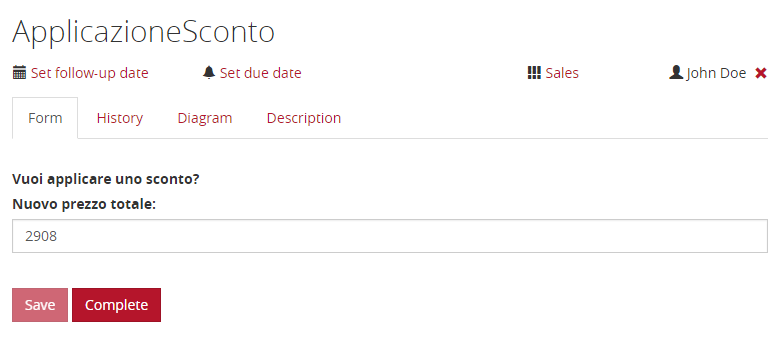
\includegraphics[scale=0.5]{immagini/formCamunda.png}\\
Si attende poi l'attesa della conferma del preventivo da parte
dell'utente. Si noti che i messaggi tra utente e sistema non sono stati
gestiti, a causa di una serie di problemi elencati nelle conclusioni.
L'implementazione dello svolgimento di questi dialoghi \`e stata
affrontata nel seguente modo: viene fissato il timeout dell'attesa a due
minuti, mentre all'invio della risposta viene assegnato un timeout di un
minuto o di tre minuti. Naturalmente, la risposta verr\`a ricevuta solo
nel primo caso.
Tale meccanismo viene utilizzato per tutte le interazioni con l'utente.
Tornando alla conferma del preventivo, l'utente (fittizio) pu\`o
rispondere anche con un rifiuto, tramite una decisione pseudo-randomica
come visto in precedenza.

Il resto del processo prevede l'interazione con i servizi Jolie, come
descritti nella sezione apposita.

Infine \`e necessario soffermarsi su due sotto-progetti di servizio,
\linebreak {\tt CommonObjects} e {\tt JolieWrapper}. {\tt CommonObjects}
contiene le classi per la serializzazione e la deserializzazione degli
ordini, mentre {\tt JolieWrapper} contiene la gestione dell'interazione
con i servizi Jolie.
